% Generated by LitigCharts.PublicationFigures. Captions and provenance are sidecars.
\documentclass[10pt,tikz,border=5pt]{standalone}
\usepackage{lmodern}
\usetikzlibrary{patterns,patterns.meta}
\begin{document}
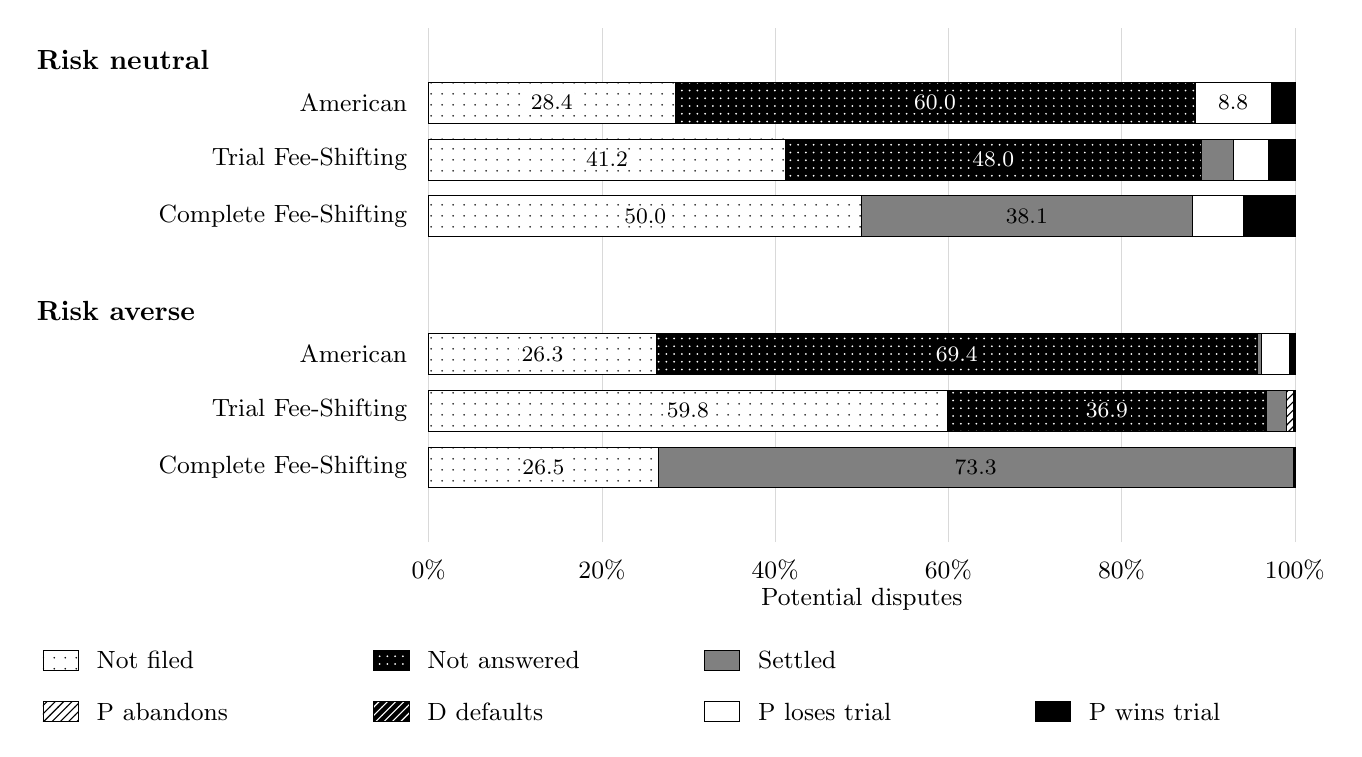
\begin{tikzpicture}[font=\small]\draw[black!15,line width=.2pt] (5.1,.65) -- (5.1,7.18);
\node[anchor=north] at (5.1,.55) {0\%};
\draw[black!15,line width=.2pt] (7.3,.65) -- (7.3,7.18);
\node[anchor=north] at (7.3,.55) {20\%};
\draw[black!15,line width=.2pt] (9.5,.65) -- (9.5,7.18);
\node[anchor=north] at (9.5,.55) {40\%};
\draw[black!15,line width=.2pt] (11.7,.65) -- (11.7,7.18);
\node[anchor=north] at (11.7,.55) {60\%};
\draw[black!15,line width=.2pt] (13.9,.65) -- (13.9,7.18);
\node[anchor=north] at (13.9,.55) {80\%};
\draw[black!15,line width=.2pt] (16.1,.65) -- (16.1,7.18);
\node[anchor=north] at (16.1,.55) {100\%};
\node[anchor=west,font=\bfseries] at (0,6.78) {\mbox{Risk} \mbox{neutral}};
\node[anchor=east] at (4.95,6.23) {American};
\path[preaction={fill=white,draw=none},pattern={Dots[distance=4pt,radius=.35pt]},pattern color=black,draw=black,line width=.25pt] (5.1,5.97) rectangle (8.22741,6.49);
\node[text=black,fill=white,font=\footnotesize,inner sep=1pt] at (6.663705,6.23) {28.4};
\path[preaction={fill=black,draw=none},pattern={Dots[distance=2.8pt,radius=.35pt]},pattern color=white,draw=black,line width=.25pt] (8.22741,5.97) rectangle (14.831051,6.49);
\node[text=white,fill=black,font=\footnotesize,inner sep=1pt] at (11.529231,6.23) {60.0};
\path[fill=white,draw=black,line width=.25pt] (14.831051,5.97) rectangle (15.803948,6.49);
\node[text=black,fill=none,font=\footnotesize,inner sep=1pt] at (15.3175,6.23) {8.8};
\path[fill=black,draw=black,line width=.25pt] (15.803948,5.97) rectangle (16.099995,6.49);
\node[anchor=east] at (4.95,5.51) {Trial Fee-Shifting};
\path[preaction={fill=white,draw=none},pattern={Dots[distance=4pt,radius=.35pt]},pattern color=black,draw=black,line width=.25pt] (5.1,5.25) rectangle (9.629888,5.77);
\node[text=black,fill=white,font=\footnotesize,inner sep=1pt] at (7.364944,5.51) {41.2};
\path[preaction={fill=black,draw=none},pattern={Dots[distance=2.8pt,radius=.35pt]},pattern color=white,draw=black,line width=.25pt] (9.629888,5.25) rectangle (14.90848,5.77);
\node[text=white,fill=black,font=\footnotesize,inner sep=1pt] at (12.269184,5.51) {48.0};
\path[fill=black!50,draw=black,line width=.25pt] (14.90848,5.25) rectangle (15.316996,5.77);
\path[fill=white,draw=black,line width=.25pt] (15.316996,5.25) rectangle (15.769318,5.77);
\path[fill=black,draw=black,line width=.25pt] (15.769318,5.25) rectangle (16.099991,5.77);
\node[anchor=east] at (4.95,4.79) {Complete Fee-Shifting};
\path[preaction={fill=white,draw=none},pattern={Dots[distance=4pt,radius=.35pt]},pattern color=black,draw=black,line width=.25pt] (5.1,4.53) rectangle (10.60011,5.05);
\node[text=black,fill=white,font=\footnotesize,inner sep=1pt] at (7.850055,4.79) {50.0};
\path[fill=black!50,draw=black,line width=.25pt] (10.60011,4.53) rectangle (14.793882,5.05);
\node[text=black,fill=none,font=\footnotesize,inner sep=1pt] at (12.696996,4.79) {38.1};
\path[fill=white,draw=black,line width=.25pt] (14.793882,4.53) rectangle (15.446947,5.05);
\path[fill=black,draw=black,line width=.25pt] (15.446947,4.53) rectangle (16.100001,5.05);
\node[anchor=west,font=\bfseries] at (0,3.59) {\mbox{Risk} \mbox{averse}};
\node[anchor=east] at (4.95,3.04) {American};
\path[preaction={fill=white,draw=none},pattern={Dots[distance=4pt,radius=.35pt]},pattern color=black,draw=black,line width=.25pt] (5.1,2.78) rectangle (7.991713,3.3);
\node[text=black,fill=white,font=\footnotesize,inner sep=1pt] at (6.545857,3.04) {26.3};
\path[preaction={fill=black,draw=none},pattern={Dots[distance=2.8pt,radius=.35pt]},pattern color=white,draw=black,line width=.25pt] (7.991713,2.78) rectangle (15.621808,3.3);
\node[text=white,fill=black,font=\footnotesize,inner sep=1pt] at (11.806761,3.04) {69.4};
\path[fill=black!50,draw=black,line width=.25pt] (15.621808,2.78) rectangle (15.672611,3.3);
\path[fill=white,draw=black,line width=.25pt] (15.672611,2.78) rectangle (16.028522,3.3);
\path[fill=black,draw=black,line width=.25pt] (16.028522,2.78) rectangle (16.100004,3.3);
\node[anchor=east] at (4.95,2.32) {Trial Fee-Shifting};
\path[preaction={fill=white,draw=none},pattern={Dots[distance=4pt,radius=.35pt]},pattern color=black,draw=black,line width=.25pt] (5.1,2.06) rectangle (11.682961,2.58);
\node[text=black,fill=white,font=\footnotesize,inner sep=1pt] at (8.391481,2.32) {59.8};
\path[preaction={fill=black,draw=none},pattern={Dots[distance=2.8pt,radius=.35pt]},pattern color=white,draw=black,line width=.25pt] (11.682961,2.06) rectangle (15.7425,2.58);
\node[text=white,fill=black,font=\footnotesize,inner sep=1pt] at (13.712731,2.32) {36.9};
\path[fill=black!50,draw=black,line width=.25pt] (15.7425,2.06) rectangle (15.995592,2.58);
\path[preaction={fill=white,draw=none},pattern={north east lines},pattern color=black,draw=black,line width=.25pt] (15.995592,2.06) rectangle (16.077051,2.58);
\path[preaction={fill=black,draw=none},pattern={north east lines},pattern color=white,draw=black,line width=.25pt] (16.077051,2.06) rectangle (16.087449,2.58);
\path[fill=white,draw=black,line width=.25pt] (16.087449,2.06) rectangle (16.092033,2.58);
\path[fill=black,draw=black,line width=.25pt] (16.092033,2.06) rectangle (16.1,2.58);
\node[anchor=east] at (4.95,1.6) {Complete Fee-Shifting};
\path[preaction={fill=white,draw=none},pattern={Dots[distance=4pt,radius=.35pt]},pattern color=black,draw=black,line width=.25pt] (5.1,1.34) rectangle (8.013592,1.86);
\node[text=black,fill=white,font=\footnotesize,inner sep=1pt] at (6.556796,1.6) {26.5};
\path[fill=black!50,draw=black,line width=.25pt] (8.013592,1.34) rectangle (16.078858,1.86);
\node[text=black,fill=none,font=\footnotesize,inner sep=1pt] at (12.046225,1.6) {73.3};
\path[fill=white,draw=black,line width=.25pt] (16.078858,1.34) rectangle (16.097053,1.86);
\path[fill=black,draw=black,line width=.25pt] (16.097053,1.34) rectangle (16.09999,1.86);
\node at (10.6,-.08) {Potential disputes};
\path[preaction={fill=white,draw=none},pattern={Dots[distance=4pt,radius=.35pt]},pattern color=black,draw=black,line width=.25pt] (0.2,-0.98) rectangle (0.65,-0.72);
\node[anchor=west] at (0.76,-0.85) {Not filed};
\path[preaction={fill=black,draw=none},pattern={Dots[distance=2.8pt,radius=.35pt]},pattern color=white,draw=black,line width=.25pt] (4.4,-0.98) rectangle (4.85,-0.72);
\node[anchor=west] at (4.96,-0.85) {Not answered};
\path[fill=black!50,draw=black,line width=.25pt] (8.6,-0.98) rectangle (9.05,-0.72);
\node[anchor=west] at (9.16,-0.85) {Settled};
\path[preaction={fill=white,draw=none},pattern={north east lines},pattern color=black,draw=black,line width=.25pt] (0.2,-1.63) rectangle (0.65,-1.37);
\node[anchor=west] at (0.76,-1.5) {P abandons};
\path[preaction={fill=black,draw=none},pattern={north east lines},pattern color=white,draw=black,line width=.25pt] (4.4,-1.63) rectangle (4.85,-1.37);
\node[anchor=west] at (4.96,-1.5) {D defaults};
\path[fill=white,draw=black,line width=.25pt] (8.6,-1.63) rectangle (9.05,-1.37);
\node[anchor=west] at (9.16,-1.5) {P loses trial};
\path[fill=black,draw=black,line width=.25pt] (12.8,-1.63) rectangle (13.25,-1.37);
\node[anchor=west] at (13.36,-1.5) {P wins trial};
\end{tikzpicture}
\end{document}
